\documentclass{scrreprt}
\usepackage{listings}
\usepackage{underscore}
\usepackage[bookmarks=true]{hyperref}
\usepackage[utf8]{inputenc}
\usepackage[english]{babel}
\usepackage{graphicx}
%\graphicspath{{work_packages/work_package_1/static/user-manual-images/}} % path relative to root
\graphicspath{{static/user-manual-images/}}
\hypersetup{
    pdftitle={Software Requirement Specification},    % title
    pdfauthor={Training Montage},                     % author
    pdfsubject={TeX and LaTeX},                        % subject of the document
    pdfkeywords={TeX, LaTeX, graphics, images}, % list of keywords
    colorlinks=true,       % false: boxed links; true: colored links
    linkcolor=blue,       % color of internal links
    citecolor=black,       % color of links to bibliography
    filecolor=black,        % color of file links
    urlcolor=purple,        % color of external links
    linktoc=page            % only page is linked
}

\def\myversion{0.1 }
\date{}

\usepackage{hyperref}
\begin{document}

\begin{flushright}
    \rule{16cm}{5pt}\vskip1cm
    \begin{bfseries}
        \Huge{USER'S MANUAL}\\
        \vspace{.9cm}
        for\\
        \vspace{.9cm}
        COE 1186 Project\\
        \vspace{.9cm}
        \LARGE{Version \myversion approved}\\
        \vspace{.9cm}
        Prepared by:\\
        Alec Rosenbaum\\
        Aric Hudson\\
        Isaac Goss\\
        Mitch Moran\\
        Parth Dadhania\\
        \vspace{1.9cm}
        Training Montage\\
        \vspace{.9cm}
        \today\\
    \end{bfseries}
\end{flushright}

\tableofcontents


%%%%%%%%%%%%%%%%%%   CTC Start   %%%%%%%%%%%%%%%%%%%%%
\chapter{Centralized Traffic Control}

% picture(s) of overall gui
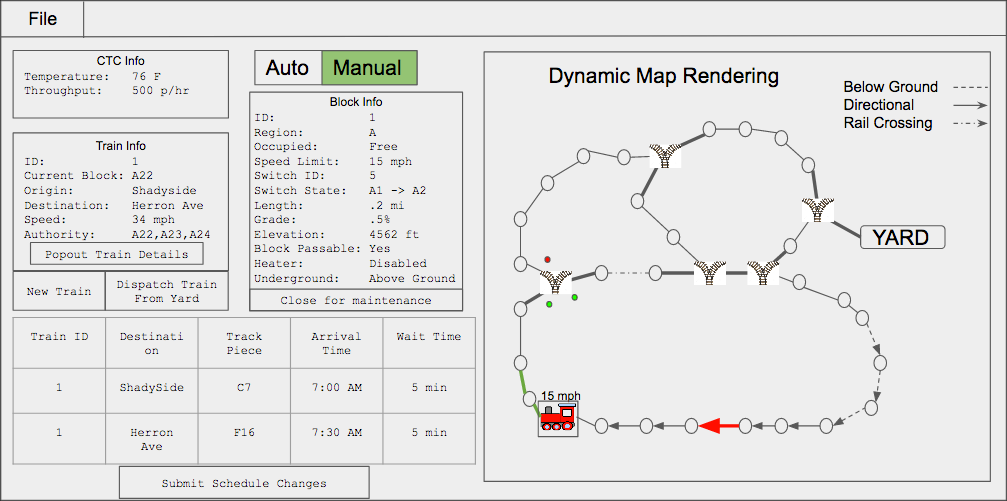
\includegraphics[width=\textwidth]{CTC-main}

\section{File Menu}
Clicking on file will show a drop down menu containing the following items:
\begin{itemize}
  \item Upload Schedule - Replace the existing schedule with a newly uploaded one
  \item Save Schedule - Export schedule with any manual changes to a file
  % Do I need an upload track option
\end{itemize}

\section{Auto/Manual Button}
\begin{center}
  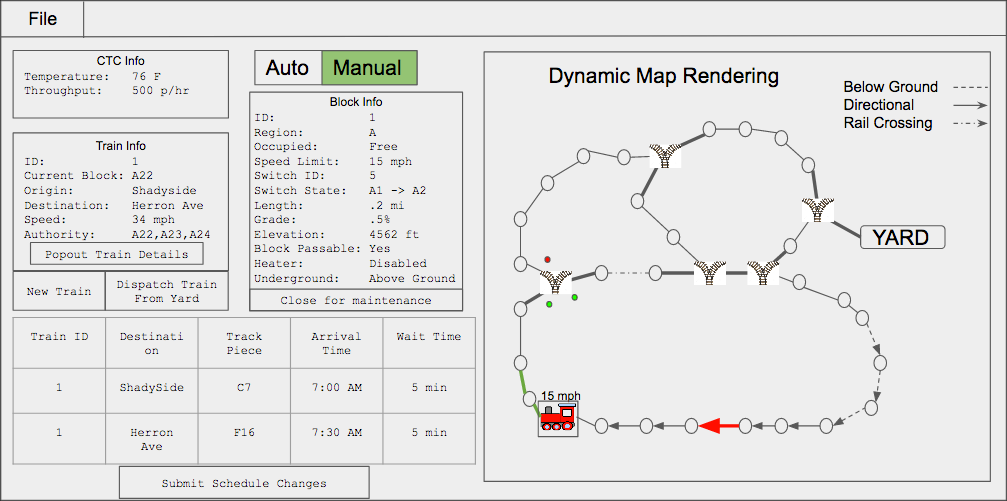
\includegraphics[trim={9cm 14.65cm 20.8cm 1.7cm},clip,width=3cm]{CTC-main}
\end{center}
% trim={<left> <lower> <right> <upper>}
Toggle between automatic and manual modes by clicking this button. In automatic mode trains 
will be dispatched according to the internal schedule. In manual mode the dispatcher must 
deploy all trains.

\section{Dynamic Map Rendering}
\begin{center}
  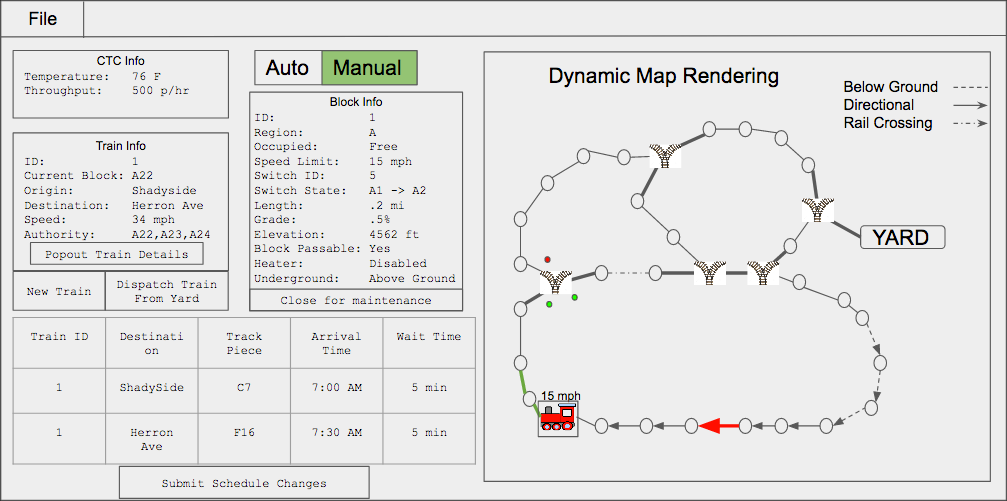
\includegraphics[trim={17cm .65cm .5cm 1.75cm},clip,width=\textwidth]{CTC-main}
\end{center}
% trim={<left> <lower> <right> <upper>}
The dynamic map rendering displays the current system state. Detailed information of each 
piece will be displayed in the relevant info boxes when a train or piece of track is clicked.

\section{CTC Info}
\begin{center}
  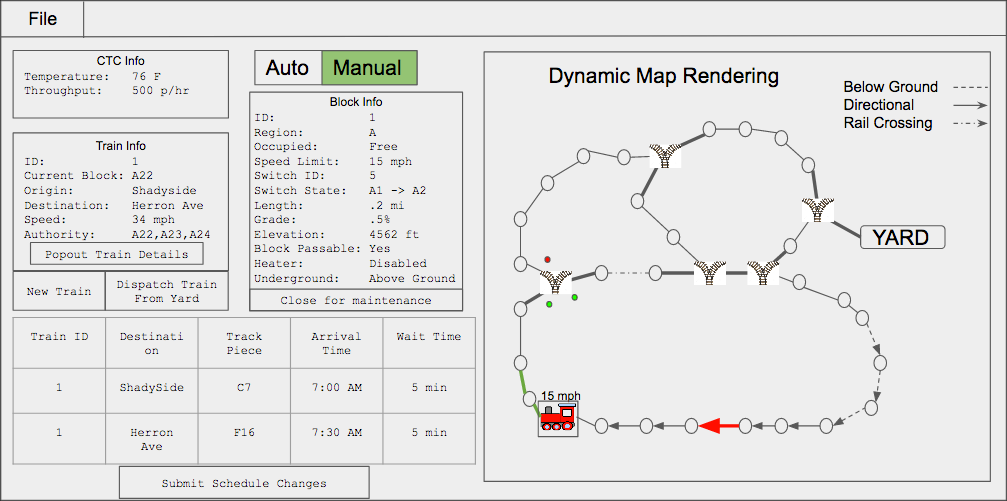
\includegraphics[trim={.45cm 13.5cm 27.45cm 1.7cm},clip,width=5cm]{CTC-main}
\end{center}
% trim={<left> <lower> <right> <upper>}
The CTC info box displays information about the currently operating system.
\begin{itemize}
  \item Temperature - Current outside temperature.
  \item Throughput - Amount of people that completed a trip within the last hour
\end{itemize}

\section{Train Info}
\begin{center}
  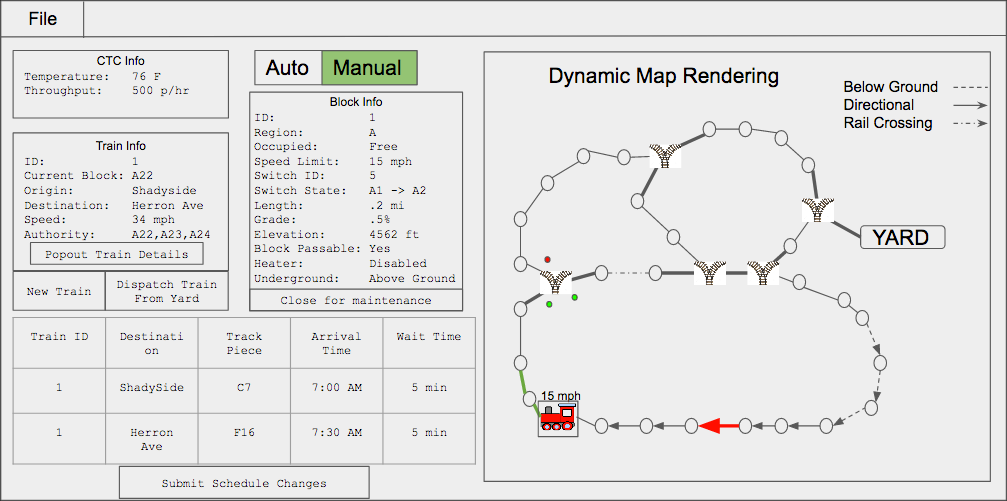
\includegraphics[trim={.45cm 6.6cm 27.45cm 4.6cm},clip,width=5cm]{CTC-main}
\end{center}
% trim={<left> <lower> <right> <upper>}
Information on a train selected in the map view will display here. The following items 
will be displayed.
\begin{itemize}
  \item Train ID - Unique ID number for the train
  \item Current Block - The current block this train occupies
  \item Origin - Location the train started at
  \item Destination - Final stop for this train
  \item Speed - Speed suggested by the CTC
  \item Authority - The permitted distance until the train must stop
\end{itemize}
The Popout Train Details button will open a new window to allow the viewing of multiple 
trains at once. This window will be explained in a later section. In manual mode, the New 
Train button will create a blank template for the dispatcher to add a new train. Once the 
new train's details are entered, Dispatch Train From Yard will send the new train. Closing 
the template window without pressing the Dispatch button will cancel the new train.

\section{Block Info}
\begin{center}
  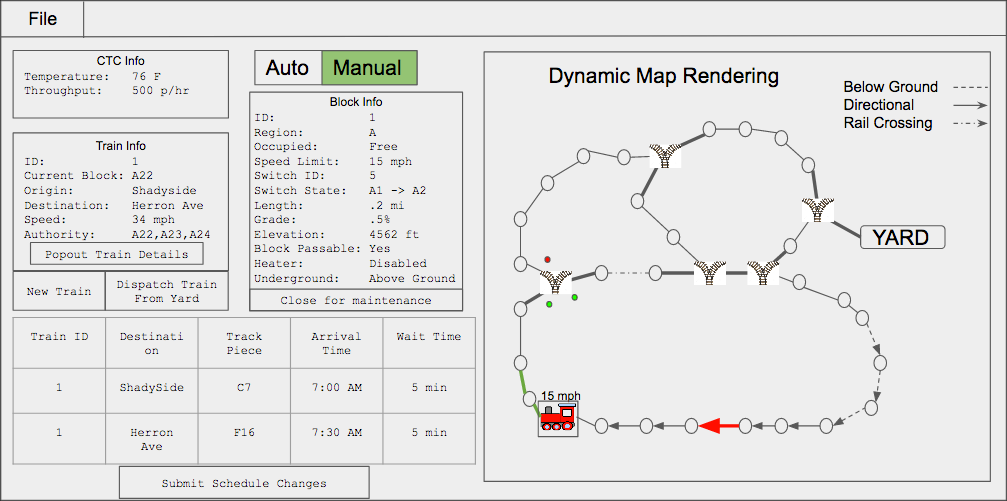
\includegraphics[trim={8.75cm 6.7cm 19.2cm 3.2cm},clip,width=5cm]{CTC-main}
\end{center}
% trim={<left> <lower> <right> <upper>}
Information on a block selected in the map view will display here. The following items 
will be displayed. Items marked with an asterisk (*) are contextual and only appear when 
relevant. 
\begin{itemize}
  \item Block ID - Together with Region forms a unique block ID
  \item Region - The region of track in which this block is located
  \item Occupied - (Yes, No) Indicates if the block is occupied or not
  \item Speed Limit - The max safe speed for that block
  \item Length - How long the block is
  \item Grade - The grade of the block
  \item Elevation - The block's elevation
  \item Block Passable - (Yes, Broken, Maintenance) If the block can be passed or the reason 
  it can't be passed
  \item Heater State - (On, Off, N/A) Indicates if the heater is on, off, or there is no heater
  \item Underground - (Yes, No) Indicates if the block is underground
  \item Light State* - (Super Green, Green, Yellow, Red) The light color currently displayed
  \item Switch ID* - A unique ID for the switch on this block
  \item Switch State* - Shows which track pieces are connected by a switch
  \item Station Name* - The name of the station on that block
  \item Number of Passengers at Station* - How many passengers are waiting at that station
  \item Railway Crossing State* - (Activated, Deactivated) When activated, trains can safely cross
\end{itemize}
The selected block can be closed or opened for maintenance by clicking the button at the 
bottom of this box.

\section{Schedule}
\begin{center}
  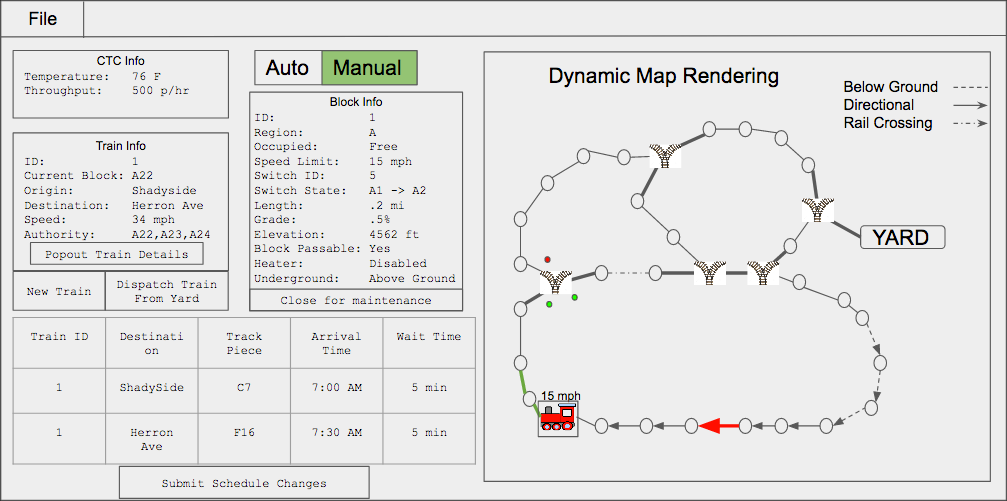
\includegraphics[trim={.45cm .08cm 18.7cm 11.15cm},clip,width=11cm]{CTC-main}
\end{center}
% trim={<left> <lower> <right> <upper>}
Displays the schedule for the whole system. Will be read-only in automatic mode and can be 
edited in manual mode. Users can select a station from the Destination column or select a specific 
block from the Track Piece column. Use the Submit button to confirm changes made to the schedule.

\section{Train Details Popout}
\begin{center}
  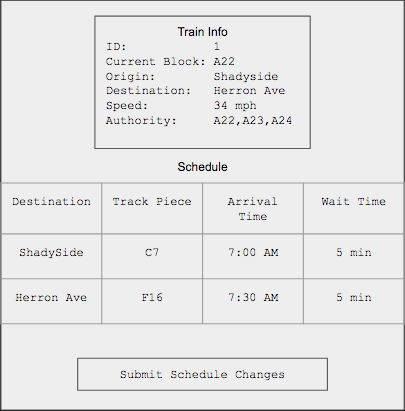
\includegraphics[width=10cm]{CTC-pop}
\end{center}
% trim={<left> <lower> <right> <upper>}
The same train information that was displayed in the main GUI will be replicated here. In 
addition the train's individual schedule can be seen here and edited while in manual mode.

%%%%%%%%%%%%%%%%%%   CTC End   %%%%%%%%%%%%%%%%%%%%%

\chapter{Track Model}

% picture(s) of overall gui
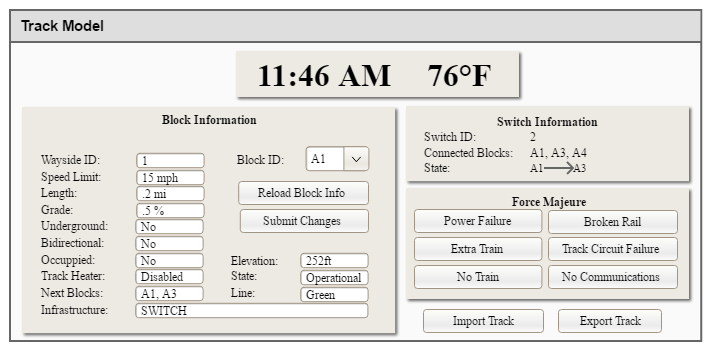
\includegraphics[width=\textwidth]{track-model}

\section{Block Information}

\begin{center}
    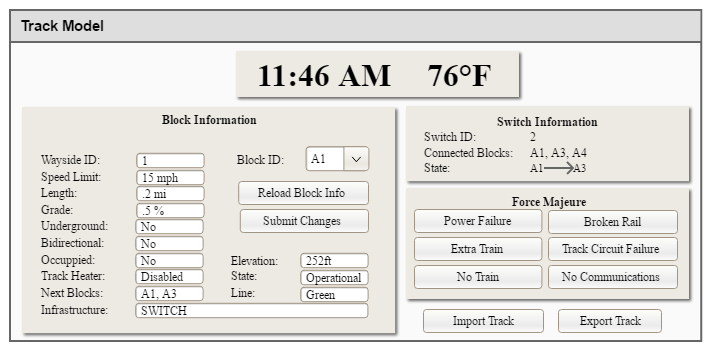
\includegraphics[trim={.5cm .5cm 11cm 3.6cm},clip,width=7.5cm]{track-model}
    % trim={<left> <lower> <right> <upper>}
\end{center}

The block information section allows the user to select a block (from a dropdown), view
stored block details, and reconfigure block details. Once the user selects a block from the
dropdown, that blocks information will be populated onto the appropriate fields. The user may
then reload the information about that block using the "Reload Block Info" button, or they
may edit any field and click the "Submit Changes" button to modify the details stored by
the Track Model.

The user may expect to see one or more of the following block states in the "State" field:
\begin{description}
    \item[Operational] The selected block is fully functional.
    \item[Broken Rail] The selected block includes a section of broken rail.
    \item[Extra Train] The selected block detects a train, when there is no train 
        actually present.
    \item[No Train] The selected block does not detect a train, when a train is present.
    \item[Power Failure] The selected block is experiencing a power failure.
    \item[No Communication] The selected block's communications aren't functional, thus no
        communication is relayed to any train present.
\end{description}

\section{Switch Information}

\begin{center}
    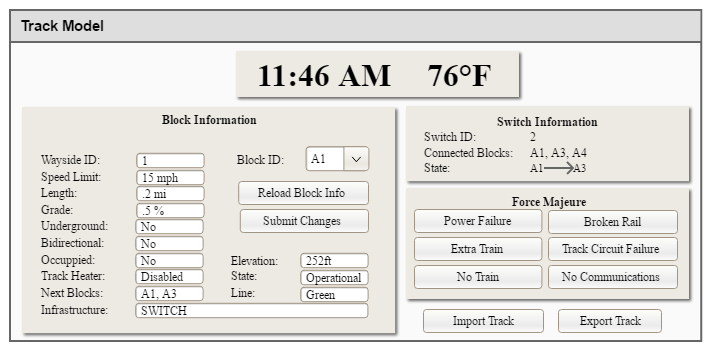
\includegraphics[trim={14.2cm 5.75cm .5cm 3.6cm},clip,width=6cm]{track-model}
    % trim={<left> <lower> <right> <upper>}
\end{center}

If there is a switch connected to the selected block, details will be presented in
this section. Details include:
\begin{itemize}
    \item Switch ID
    \item Connected Blocks
    \item Switch State
\end{itemize}

\section{Force Majeure}

\begin{center}
    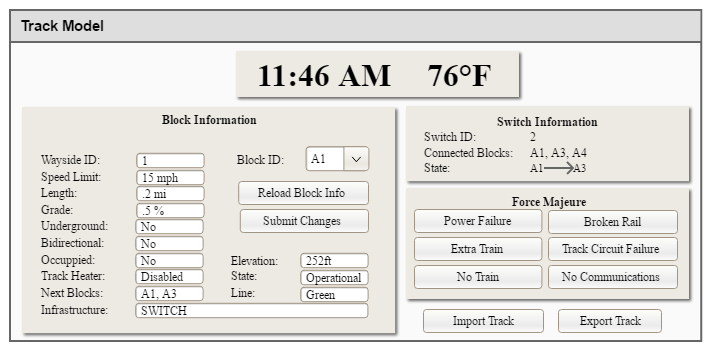
\includegraphics[trim={14.2cm 1.75cm .5cm 6.5cm},clip,width=7.5cm]{track-model}
    % trim={<left> <lower> <right> <upper>}
\end{center}

All options for causing Force Majeure failures are presented here. When the user clicks
an option, the Force Majeure failure is applied to the selected block.

\section{Track Import and Export}

\begin{center}
    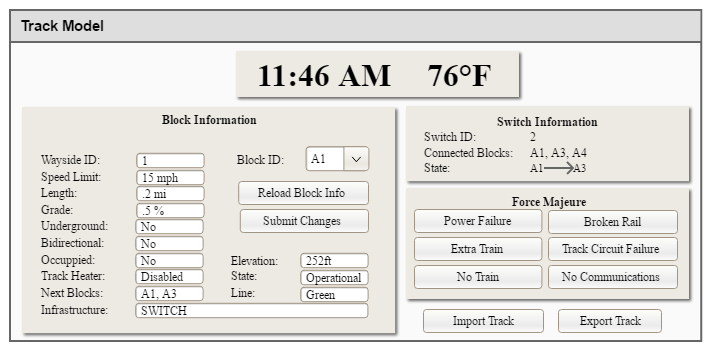
\includegraphics[trim={14.2cm .5cm .5cm 10.75cm},clip,width=7.5cm]{track-model}
    % trim={<left> <lower> <right> <upper>}
\end{center}

Track import and export options are presented here. The "Import Track" button allows
the entire track to be replaced with an imported track. The "Export Track" button allows
the entire track to be exported based on its current state.

\end{document}
